\chapter{Development}

\label{ch:Development}

\setlength{\parindent}{4em}
\setlength{\parskip}{1em}
\renewcommand{\baselinestretch}{1.5}

\section{Chamber for the experiment}
Because we use the light to stimulate the subject,so we need to have the light that enters the subject's retina are only from the stimulus, also help to increase an accuracy of the result. Therefore, we use the experiment chamber from our senior project.\\
\begin{figure}[ht]
	\centering
	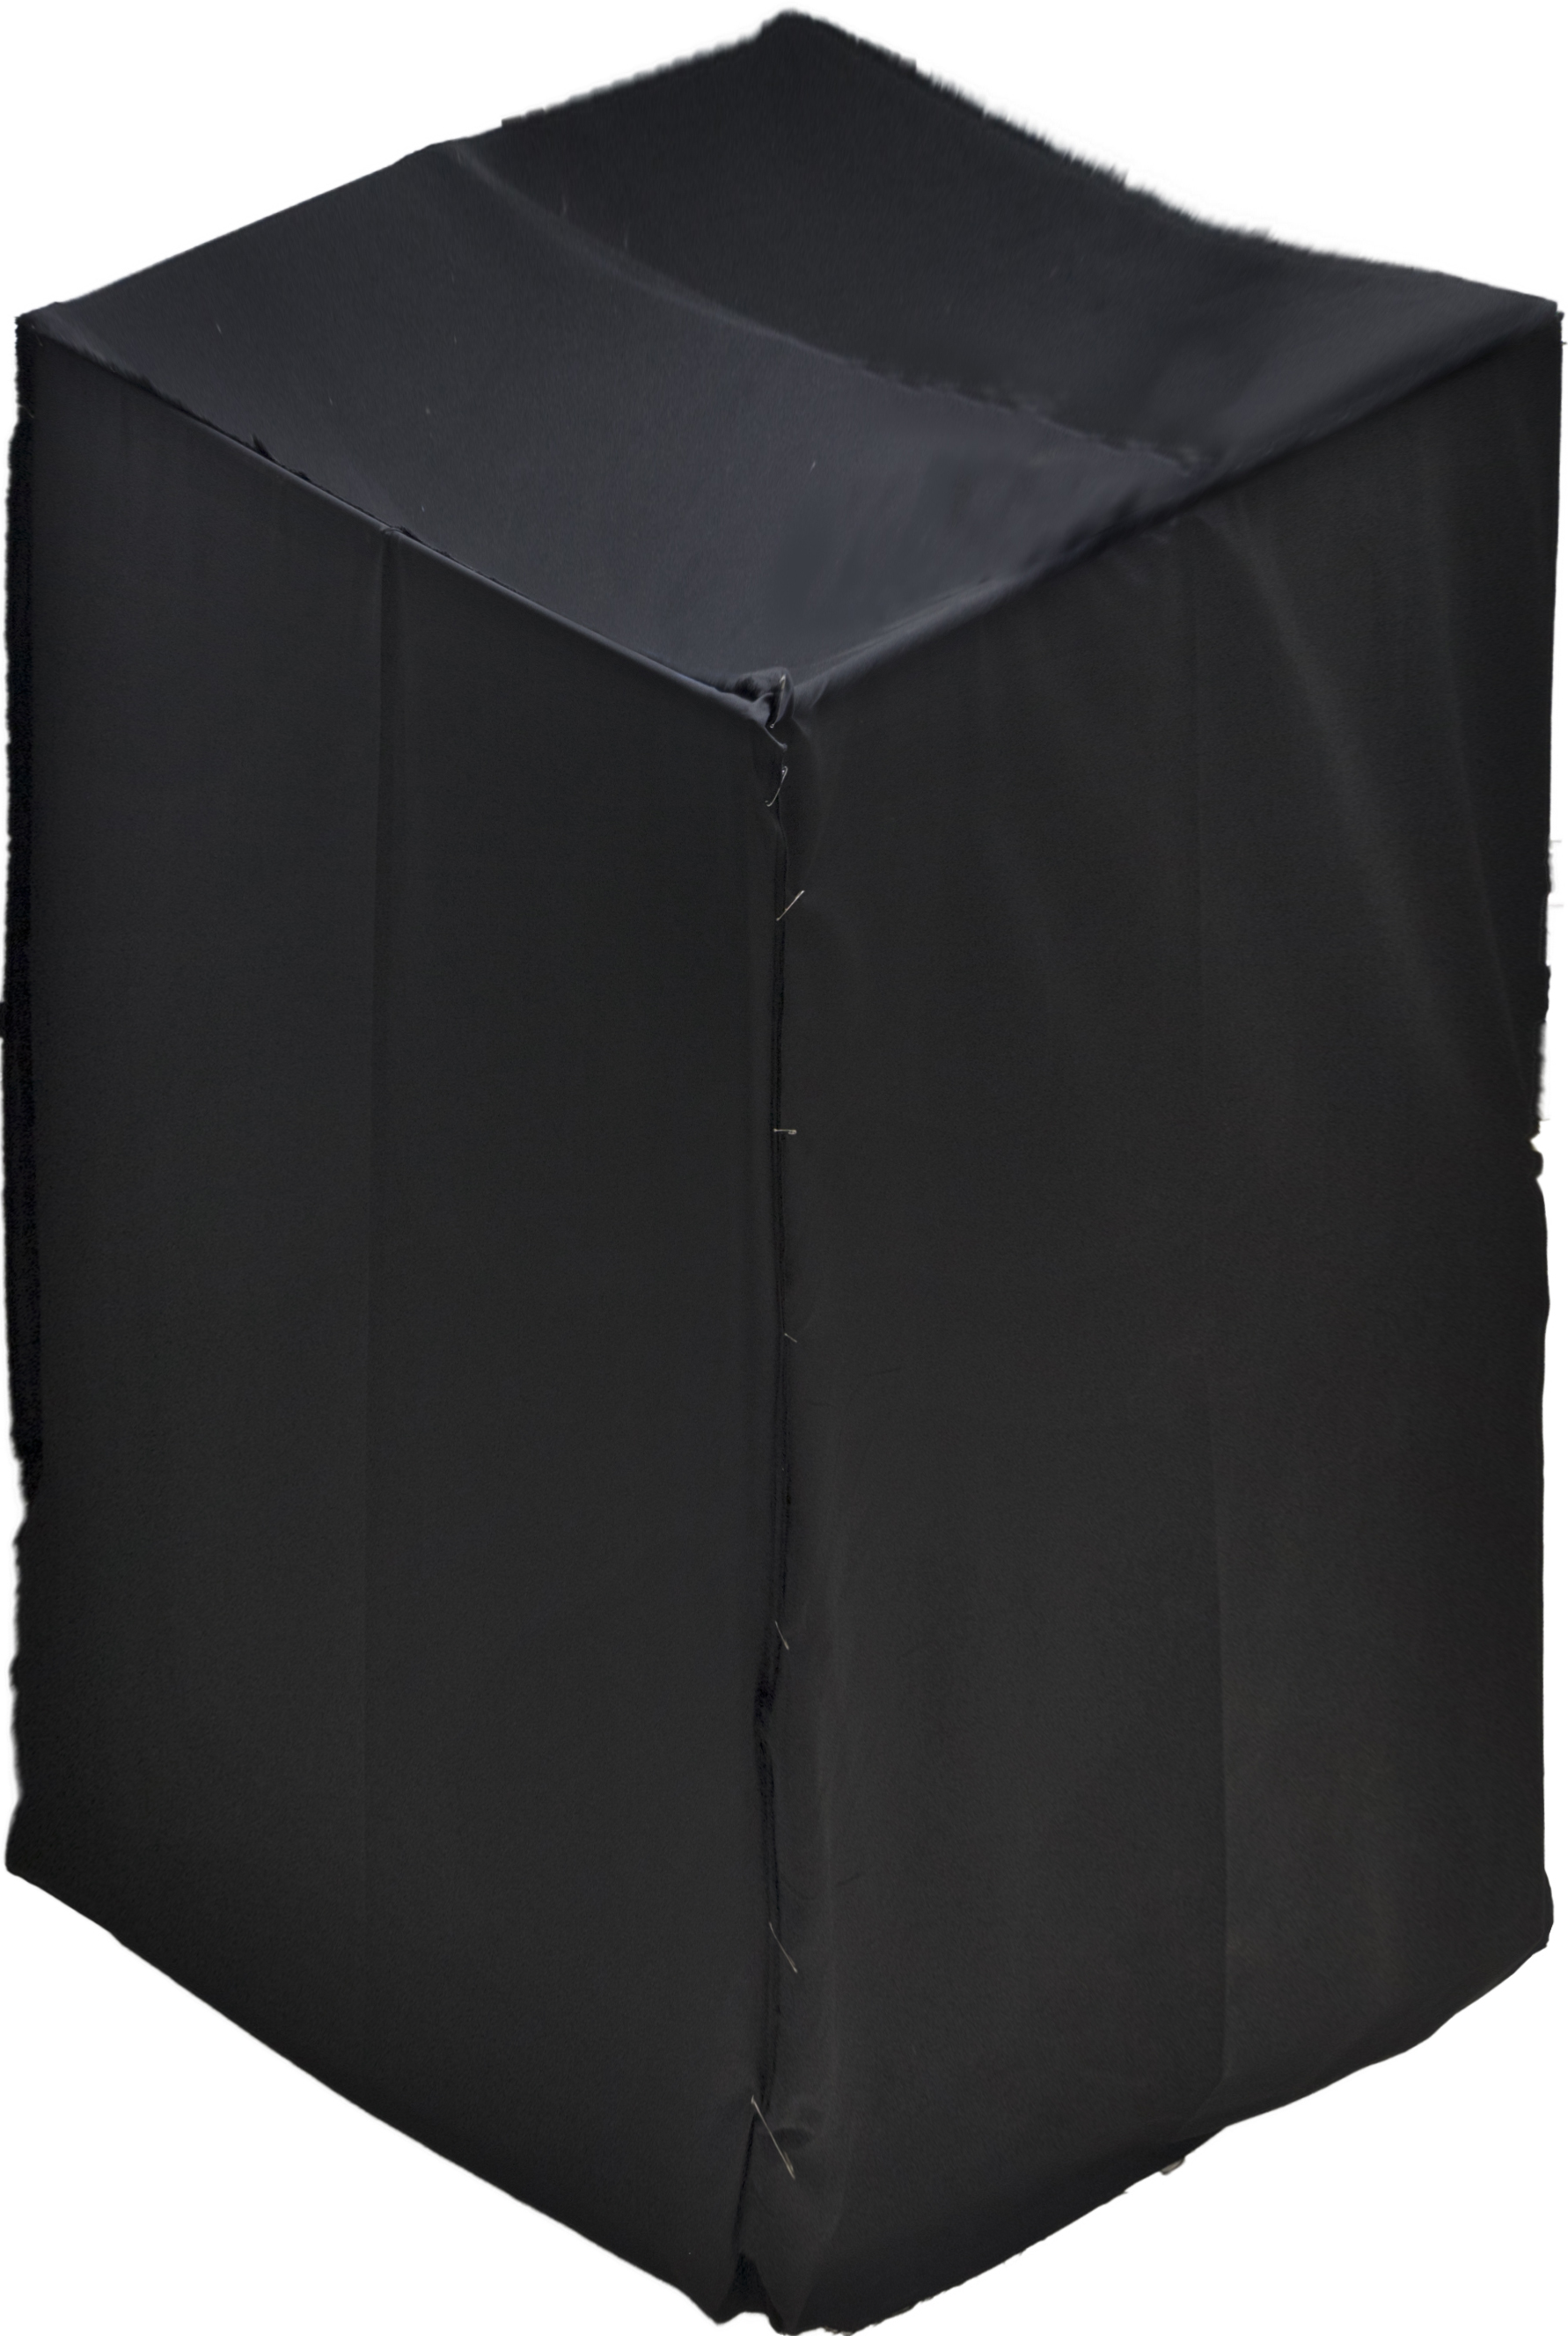
\includegraphics[width=0.4\textwidth]{chapter6/blackbox.jpg}
	\caption{Experiment Chamber}
\end{figure}
The chamber is made from PVC pipeline and black fabric. The dimension of the chamber is W x D x H : 1.5 x 1.5 x 1.9 meters.\\
\begin{figure}[ht]
	\centering
	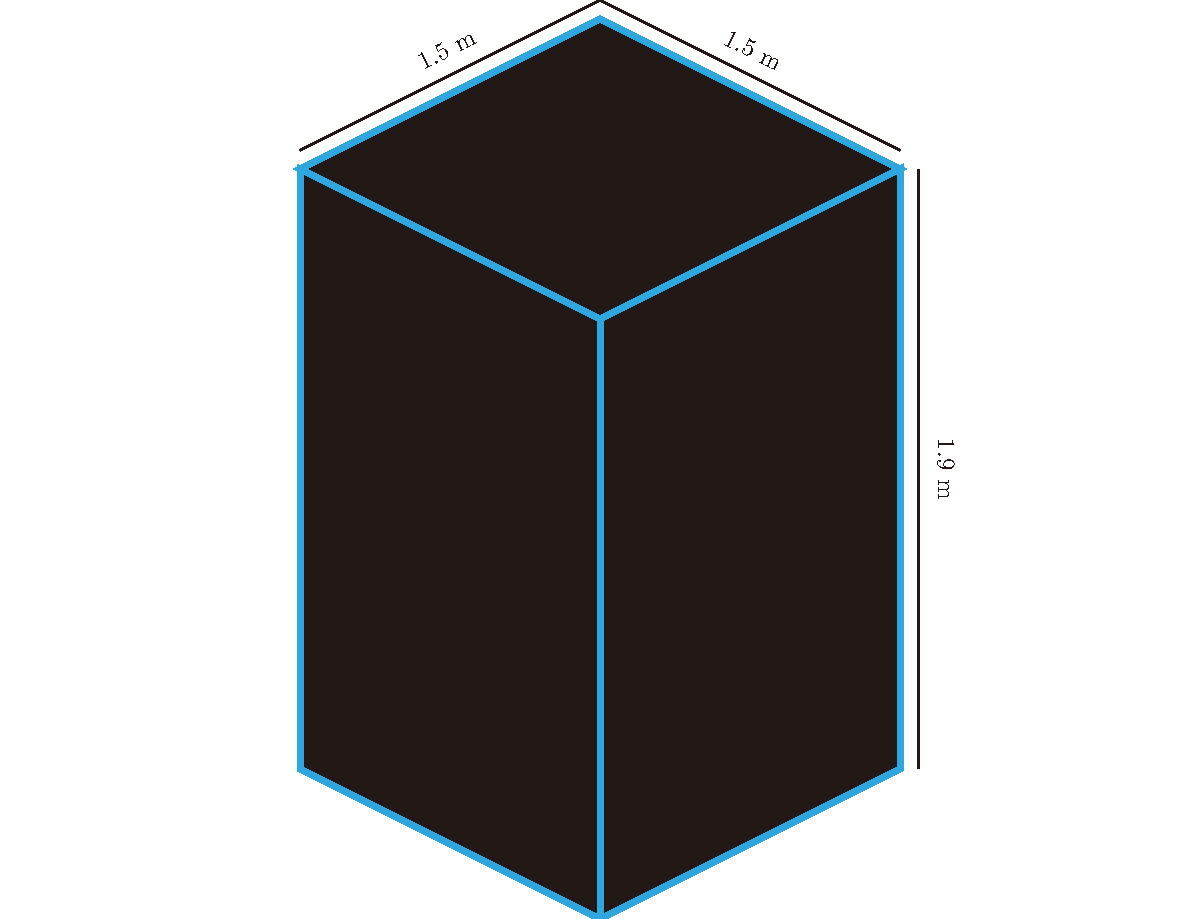
\includegraphics[width=0.8\textwidth]{chapter6/dark_wire.pdf}
	\caption{Experiment Chamber dimension}
\end{figure}
Inside the chamber, it is dark, only light from the visual stimulator are allowed. The subject will have a chair to sit on. The visual stimulator is set on the table. The distance between the visual stimulator and subject's eye is 30 cm. the subject will sit on a chair, the visual stimulator will start its work. the subject's EEG will transmit wirelessly to the computer to processing and classification. After the classification process done, it will do the function that it is assign to. \\
\begin{figure}[ht]
	\centering
	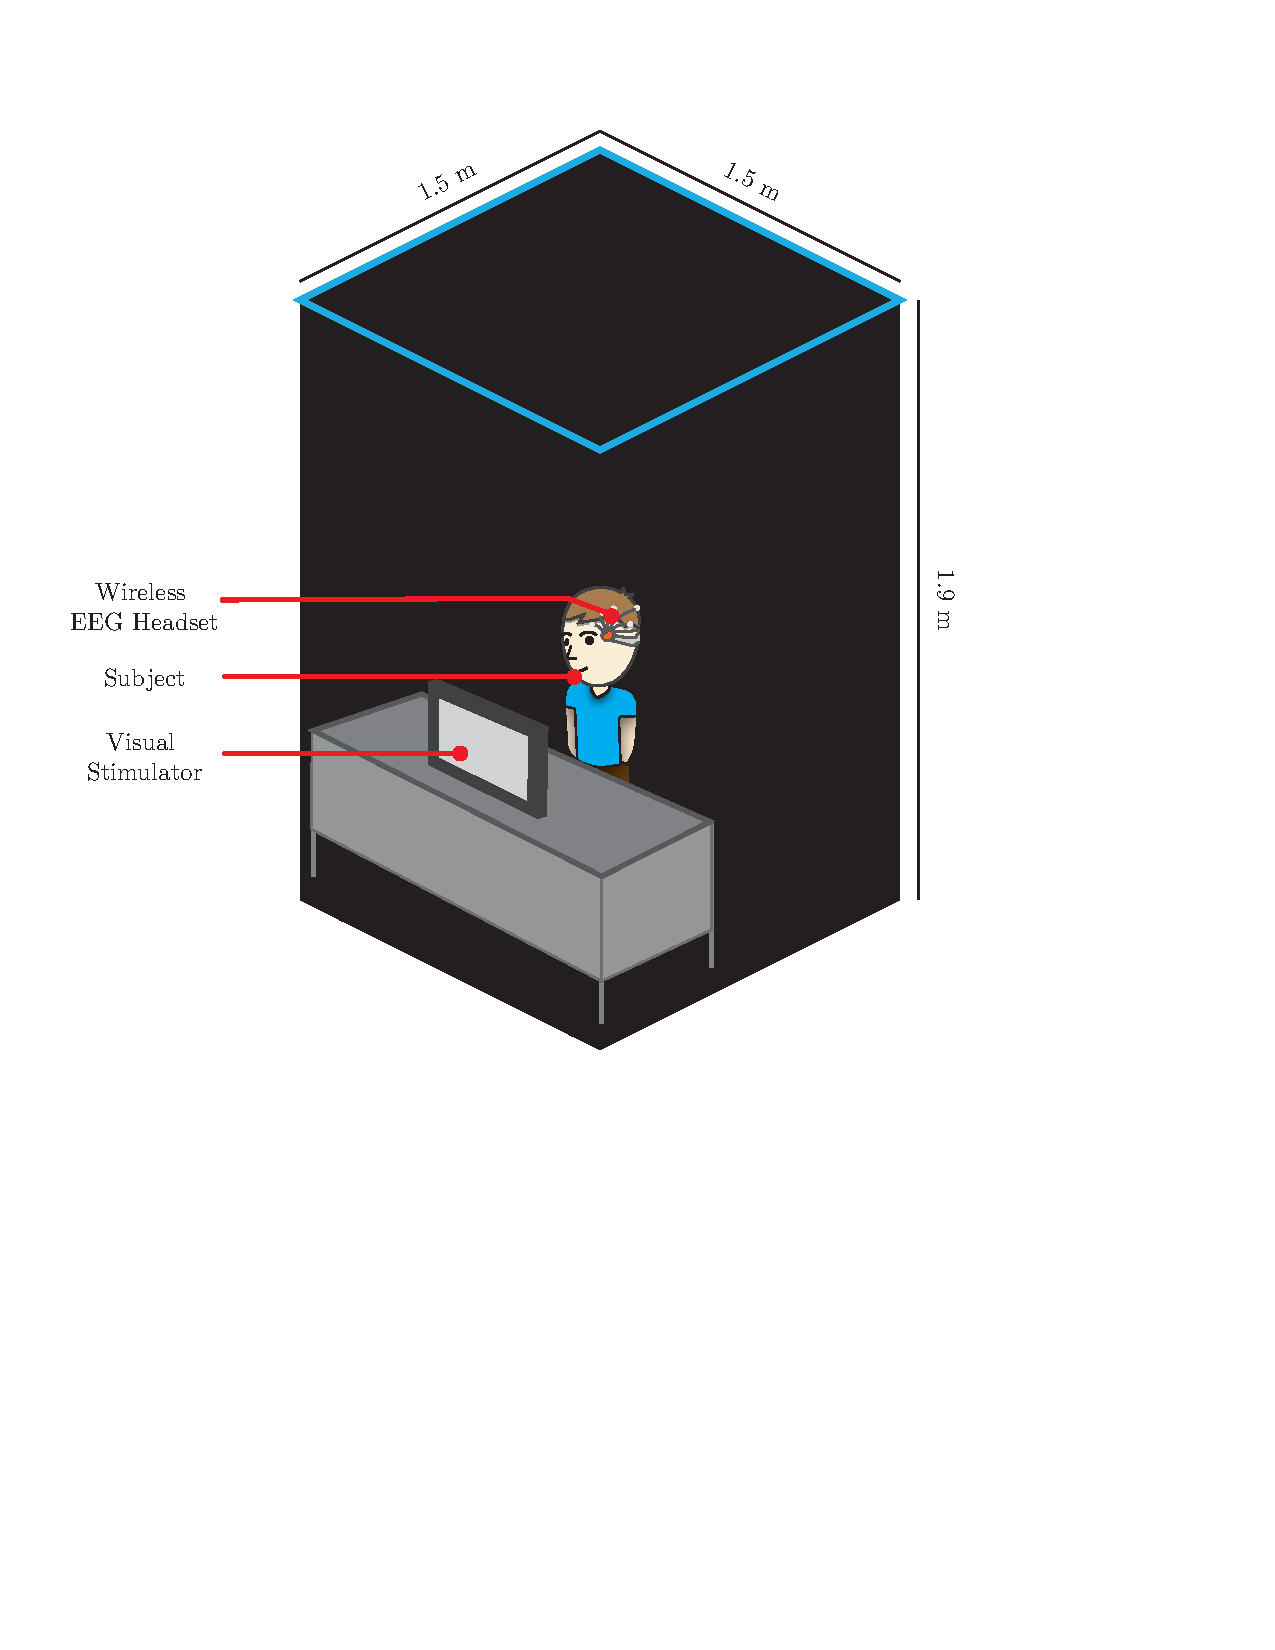
\includegraphics[width=0.8\textwidth]{chapter6/dark_wire_inside.pdf}
	\caption{Inside experiment Chamber}
\end{figure}

\begin{figure}[ht]
	\centering
	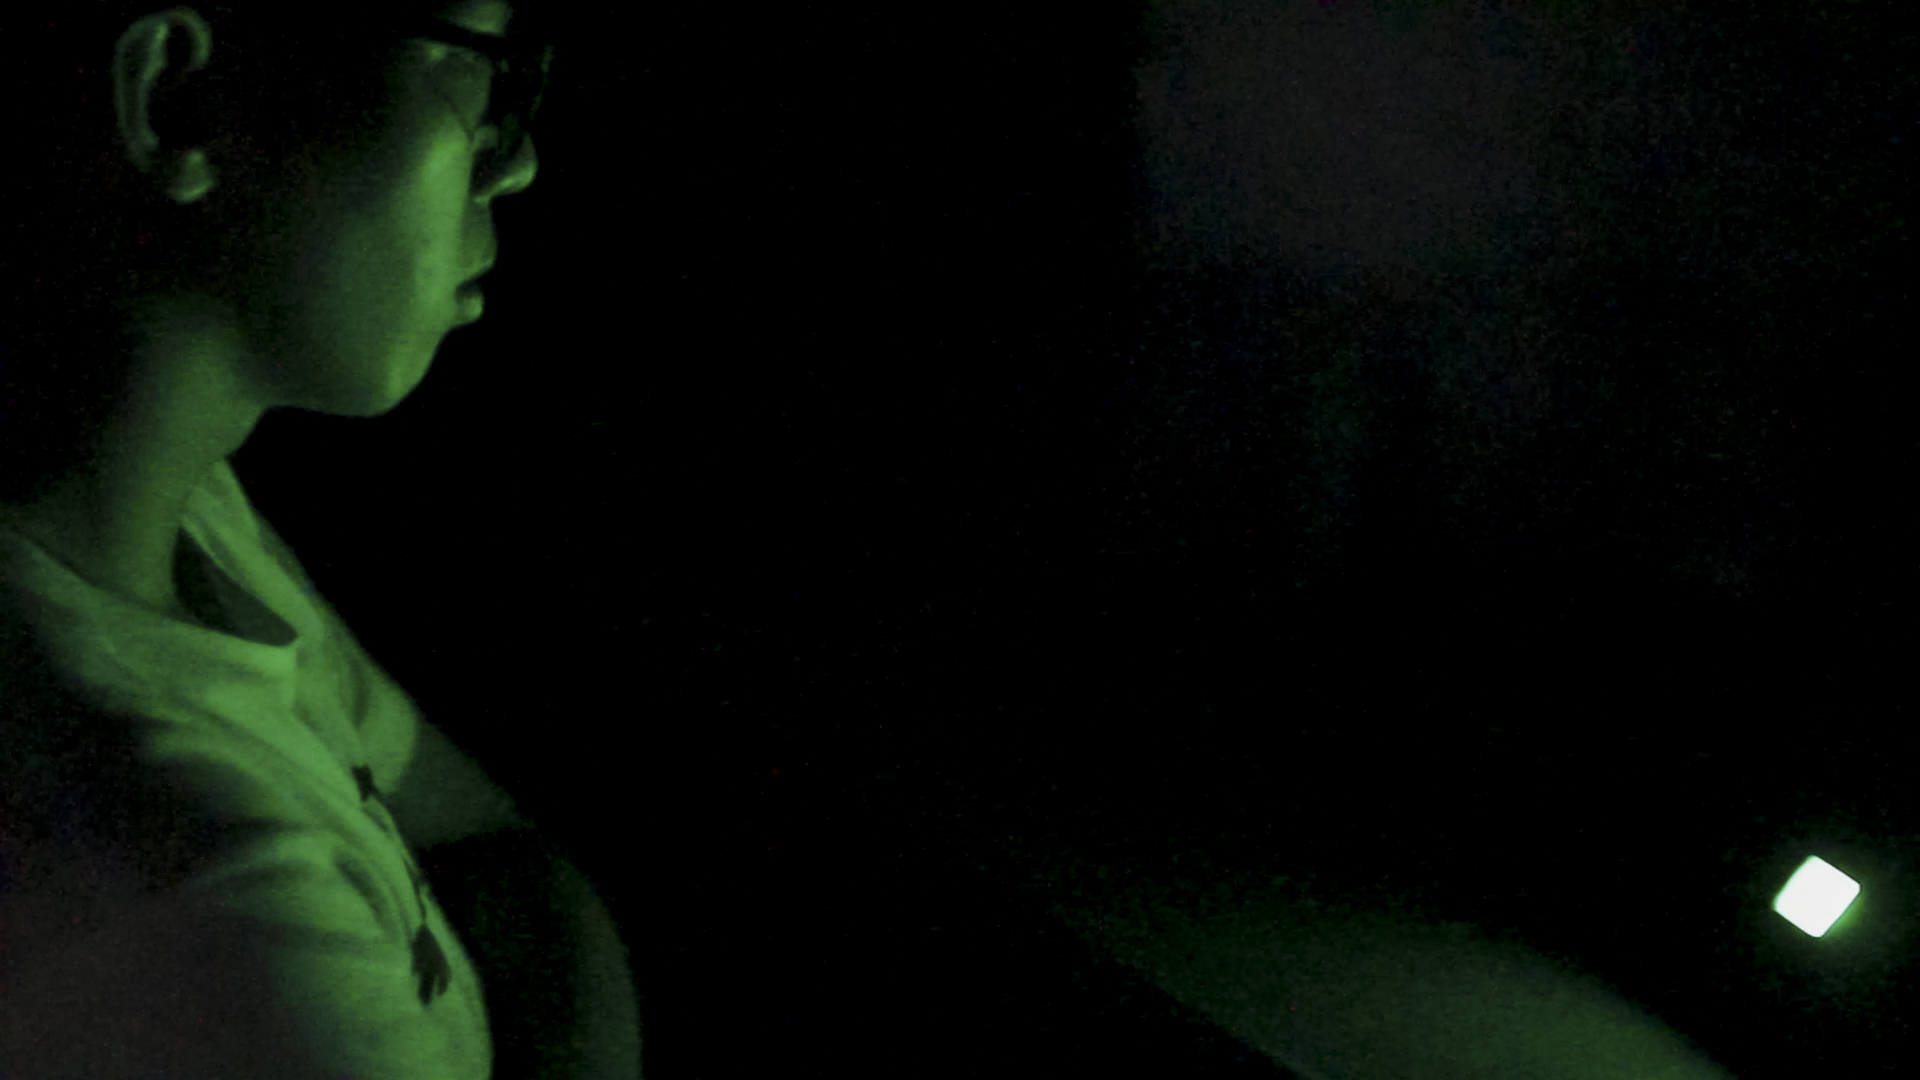
\includegraphics[width=0.8\textwidth]{chapter6/experi.jpg}
	\caption{While in experiment}
\end{figure}

\section{Visual stimulator}



\begin{figure}[ht]
	\centering
	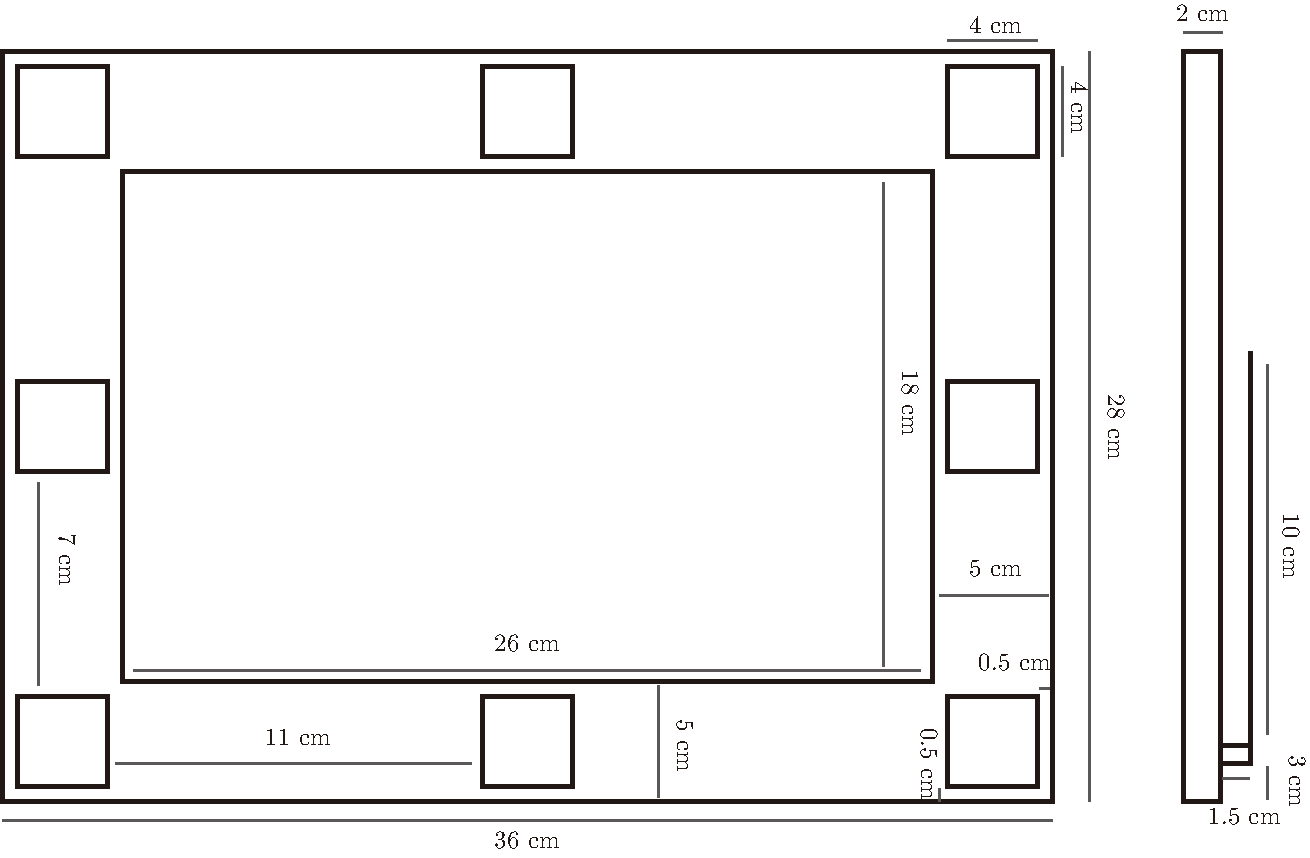
\includegraphics[width=0.7\textwidth]{chapter6/blueprint.pdf}
	\caption{Blueprint of Visual Stimulator}
\end{figure}

\begin{figure}[ht]
	\centering
	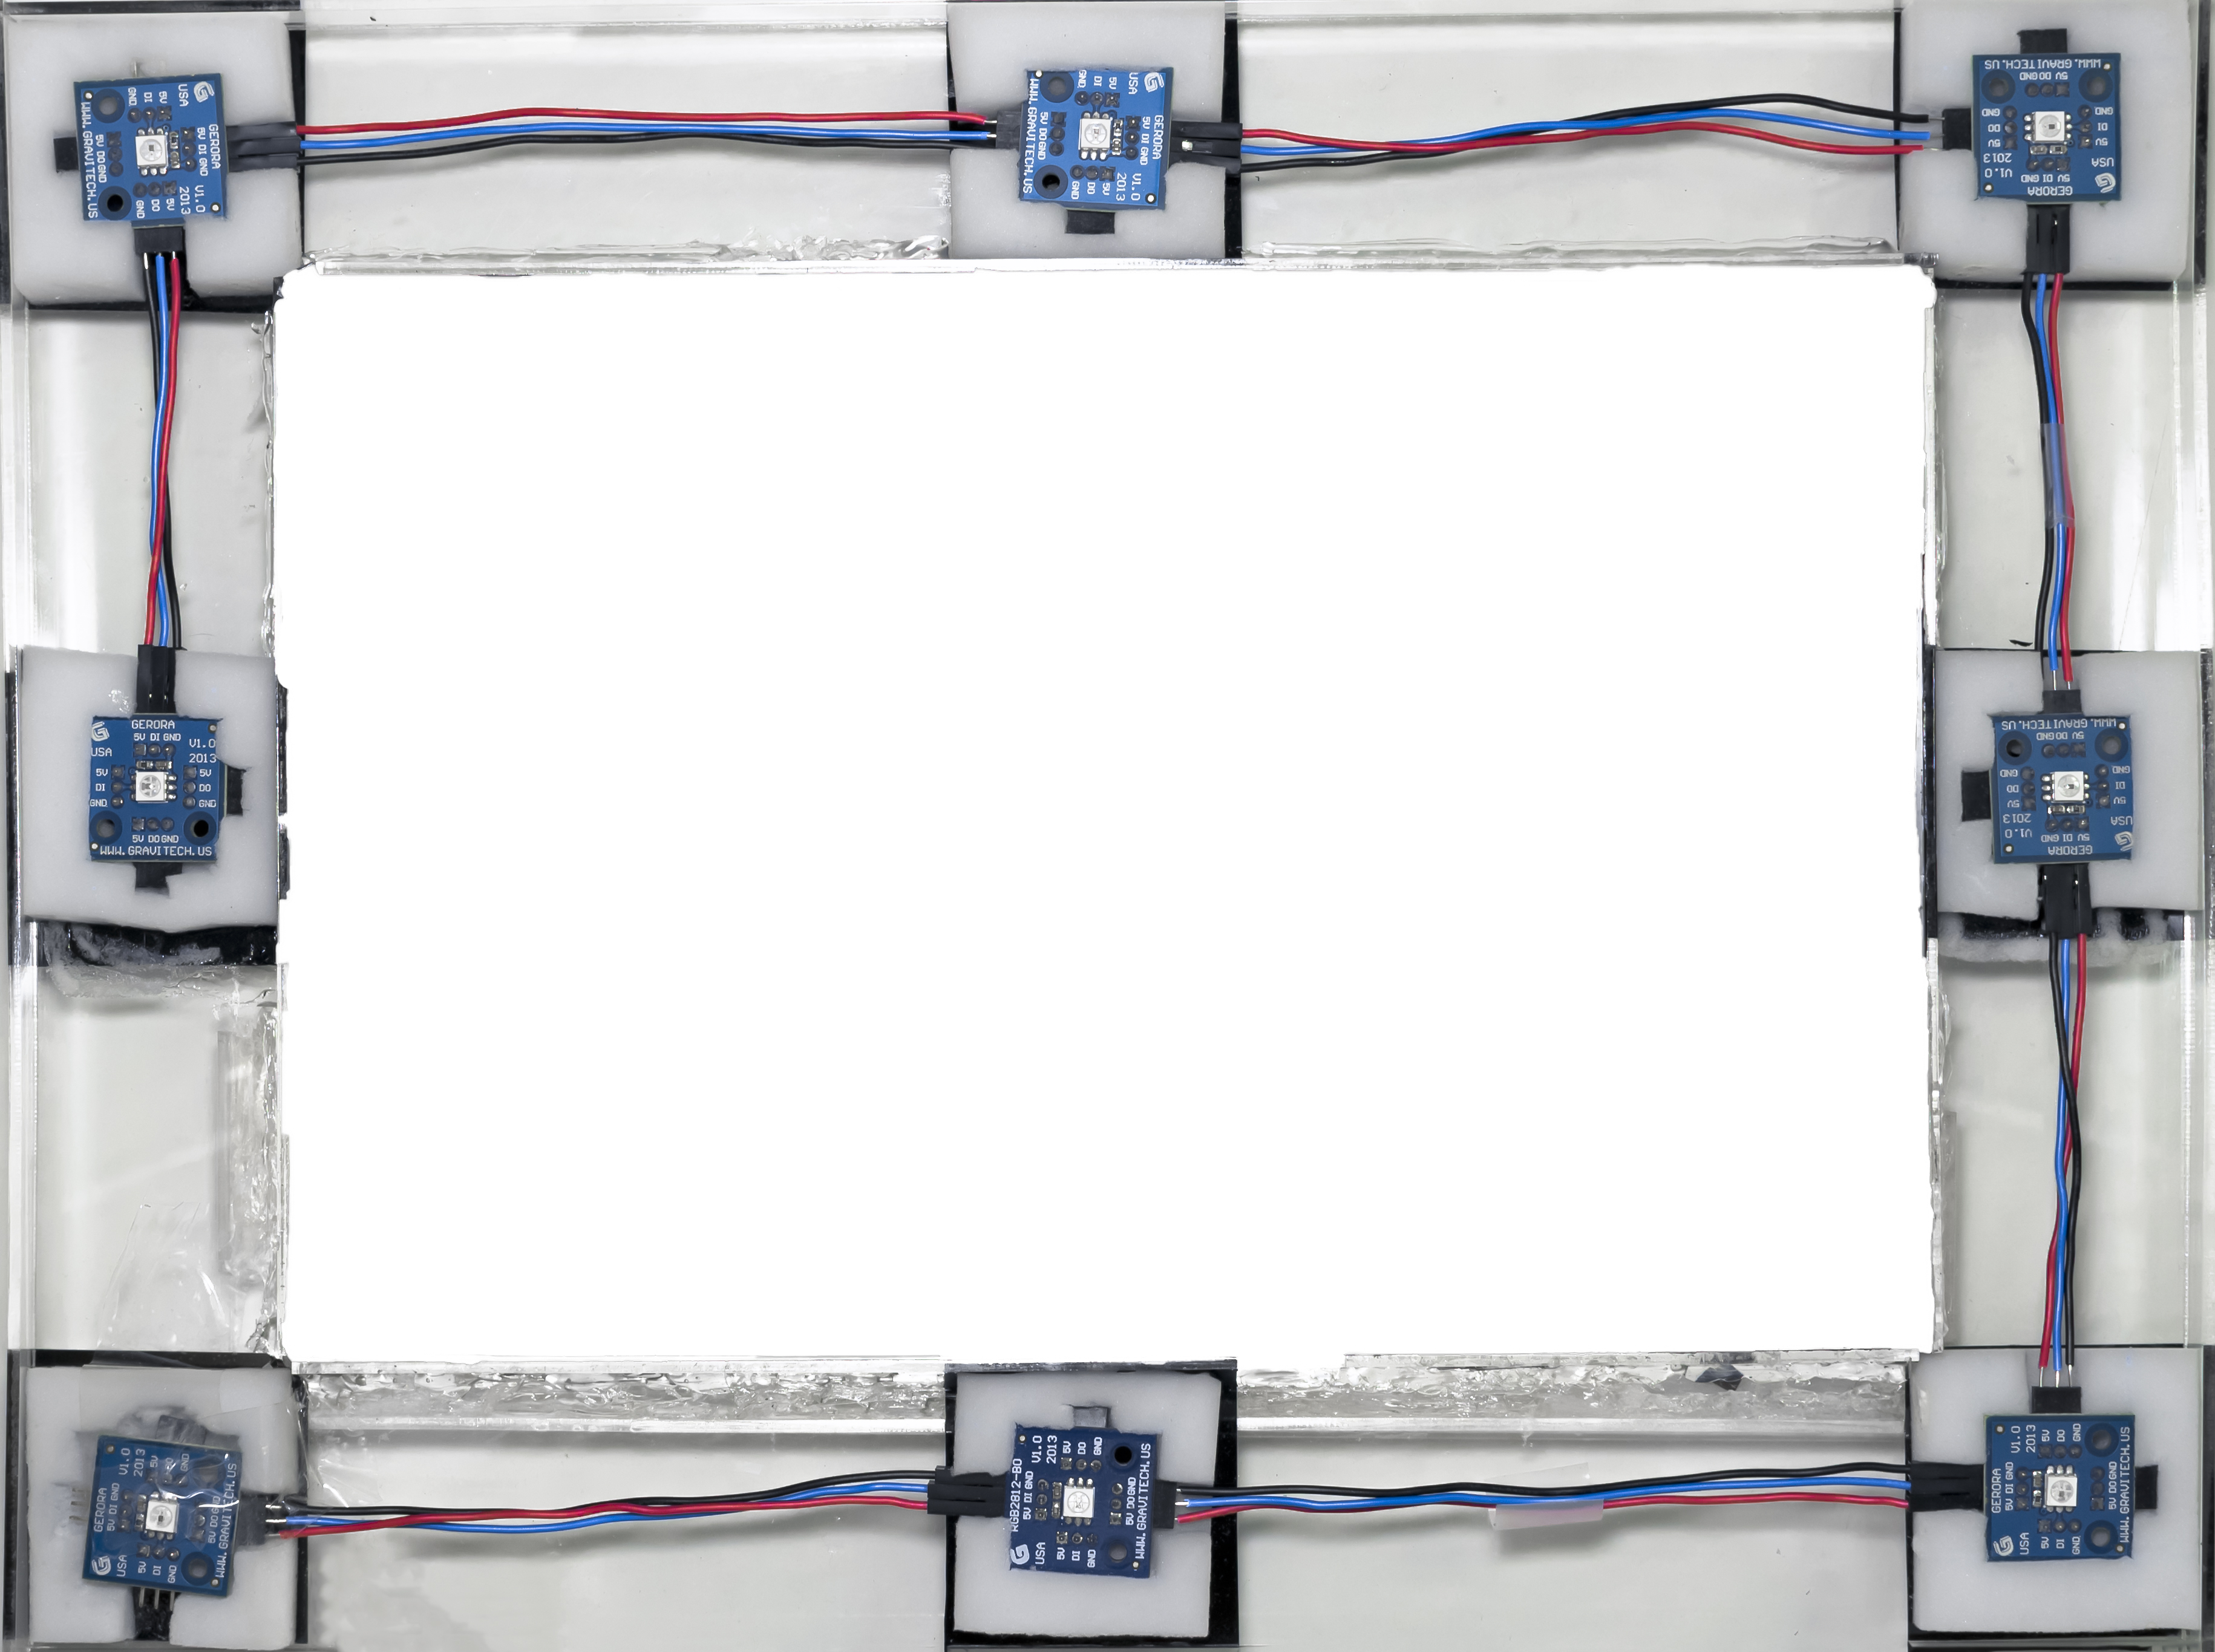
\includegraphics[width=0.7\textwidth]{chapter6/frame_LED.jpg}
	\caption{Visual Stimulator with LEDs wireing}
\end{figure}

\begin{figure}[ht]
	\centering
	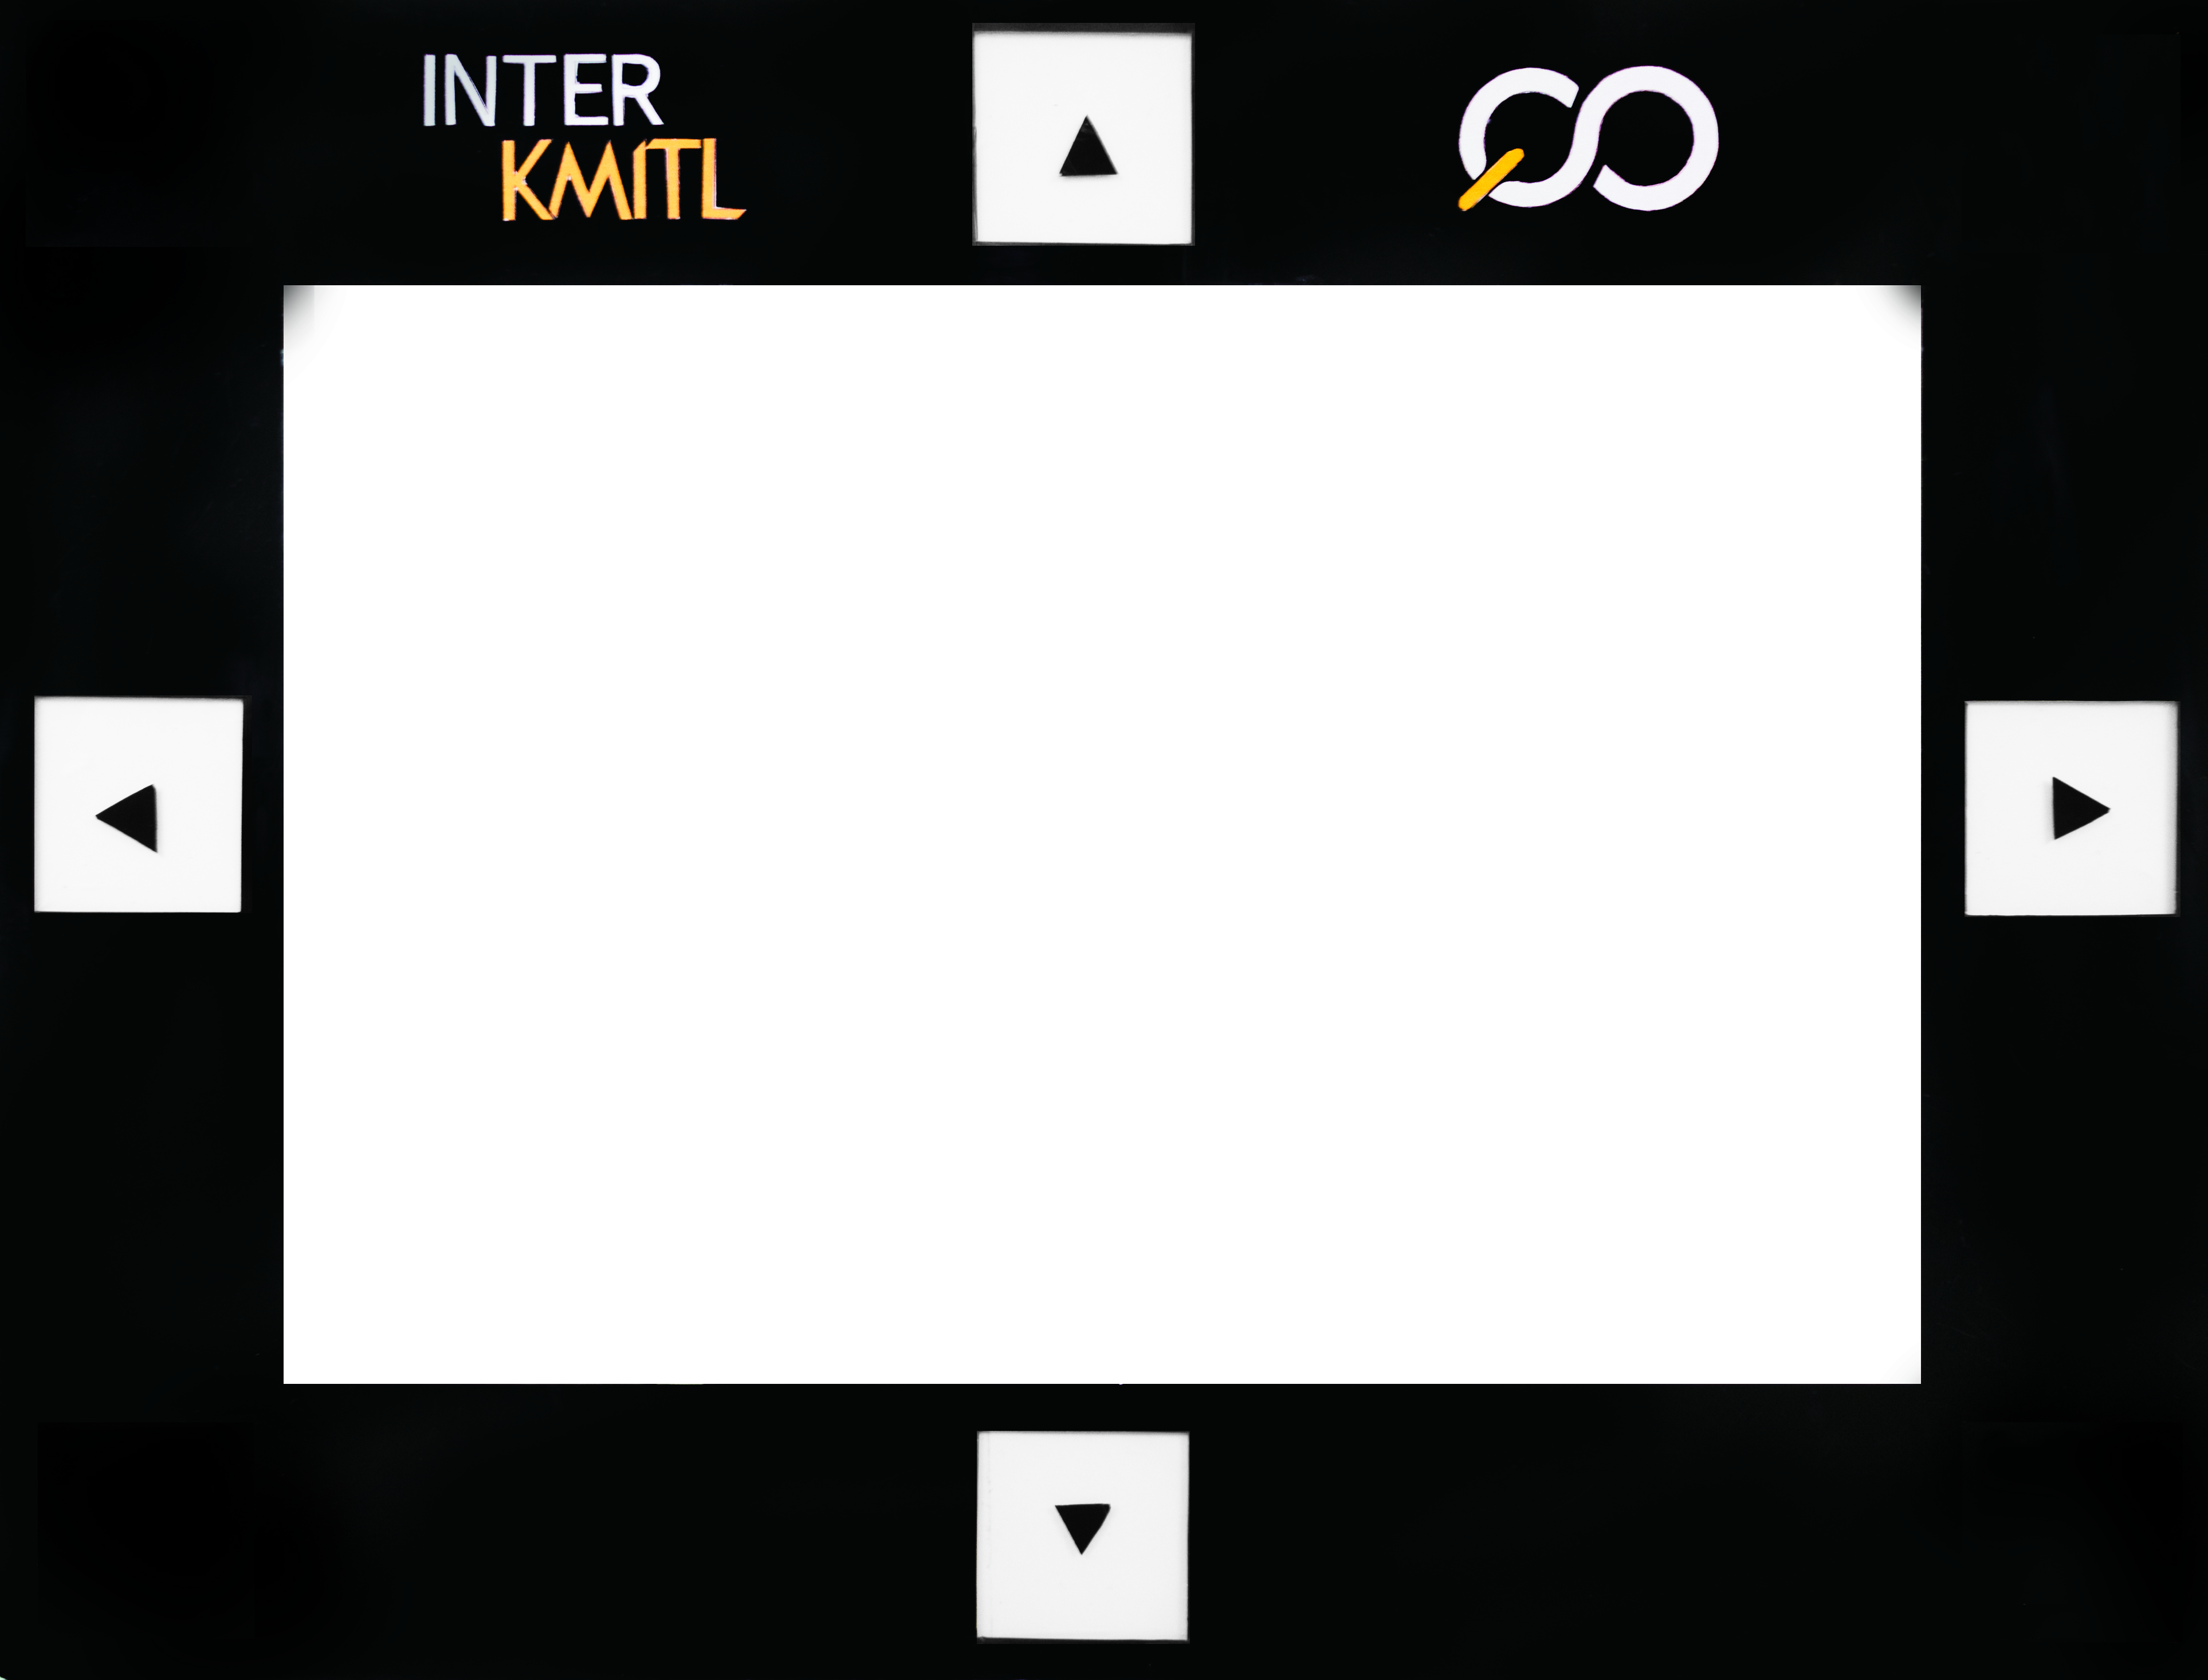
\includegraphics[width=0.7\textwidth]{chapter7/frame_4.jpg}
	\caption{Visual Stimulator with four targets used for ERPs}
\end{figure}

\begin{figure}[ht]
	\centering
	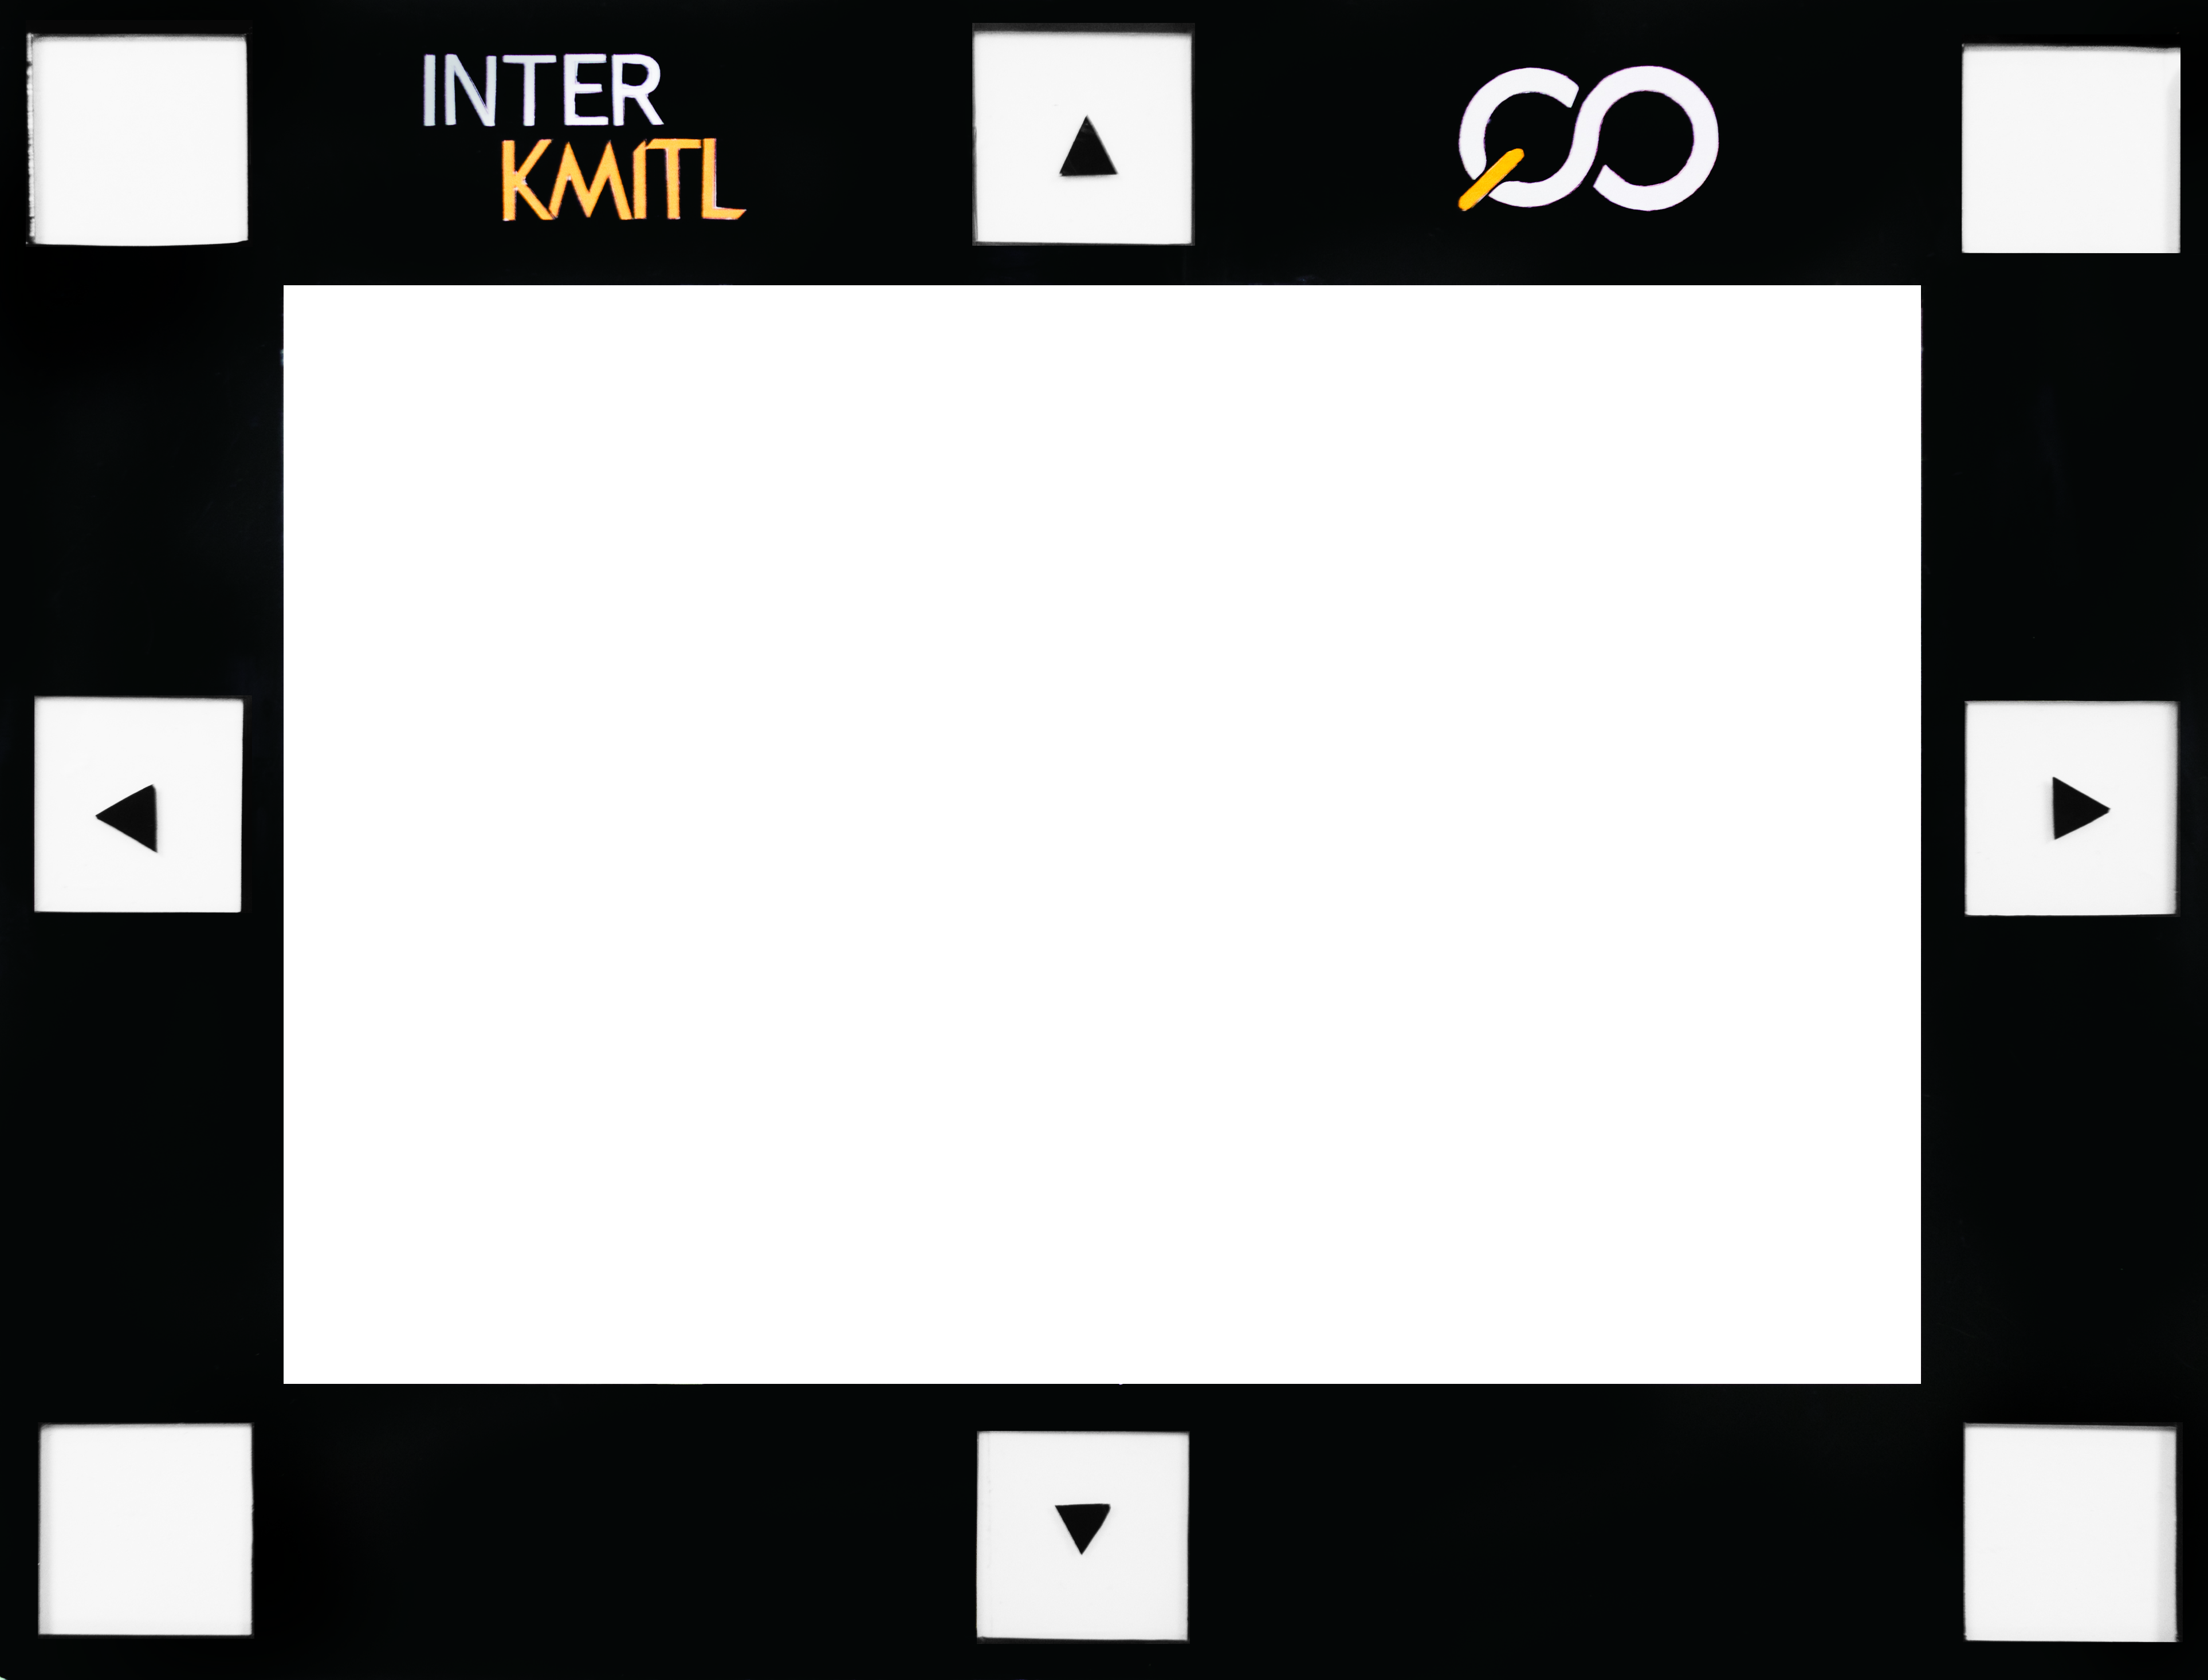
\includegraphics[width=0.7\textwidth]{chapter7/frame_8.jpg}
	\caption{Visual Stimulator with eight targets used for SSVEP}
\end{figure}

\section{Visual stimulator parameter}